\documentclass[onecolumn, draftclsnofoot,10pt, compsoc]{article}

\usepackage{graphicx}
\usepackage{amssymb}
\usepackage{amsmath}
\usepackage{amsthm}
\usepackage{pdfpages}


\usepackage{alltt}
\usepackage{float}
\usepackage{color}
\usepackage{url}

\usepackage[TABBOTCAP, tight]{}
\usepackage{enumitem}

\usepackage{geometry}
\geometry{textheight=8.5in, textwidth=6in}

%random comment

\newcommand{\cred}[1]{{\color{red}#1}}
\newcommand{\cblue}[1]{{\color{blue}#1}}

\usepackage{hyperref}
\usepackage{geometry}

\begin{document}
    \begin{titlepage}
    \newcommand{\HRule}{\rule{\linewidth}{0.5mm}}
    \center
    \textsc{\Large Oregon State University}\\[1.5cm]
    \textsc{\Large CS 461}\\[0.5cm]
    \textsc{\Large Fall 2017}\\[0.5cm]
    \HRule \\[0.4cm]
    { \huge \bfseries Tech Review AgBizClimate\textcopyright}\\[0.4cm] % Title of your document
    \HRule \\[1.5cm]
    \begin{minipage}{0.4\textwidth}
        \begin{flushleft} \large
        \emph{Author:}\\
        Thomas Noelcke
        \end{flushleft}
    \end{minipage}
    \begin{minipage}{0.4\textwidth}
        \begin{flushright} \large
        \emph{Instructor:} \\
        D. Kevin McGrath\\
        Kirsten Winters
        \end{flushright}
    \end{minipage}\\[2cm]
    \begin{abstract}
    \item 
		The purpose of this document is to research and consider different technical options for our application. In this document we research different options for data storage, HTTP request frame works, and testing frameworks. We will consider three possible choices for each section of the application. For each of these options we will weight the pros and cons of each. After comparing the different options we will select the option we would like to use for the \textit{AgBizClimate} application. We have divided our application into 9 different section and each of us has preformed this analysis for each of the nine sections.
    \end{abstract}
    \vfill % Fill the rest of the page with whitespace
    \end{titlepage}
		\newpage
		\pagenumbering{arabic}
		\tableofcontents
		\newpage
		\clearpage
		
		\section{Shane Barrantes}
			\includegraphics{Shane/main.ps}
		
		\section{Thomas Noelcke}
			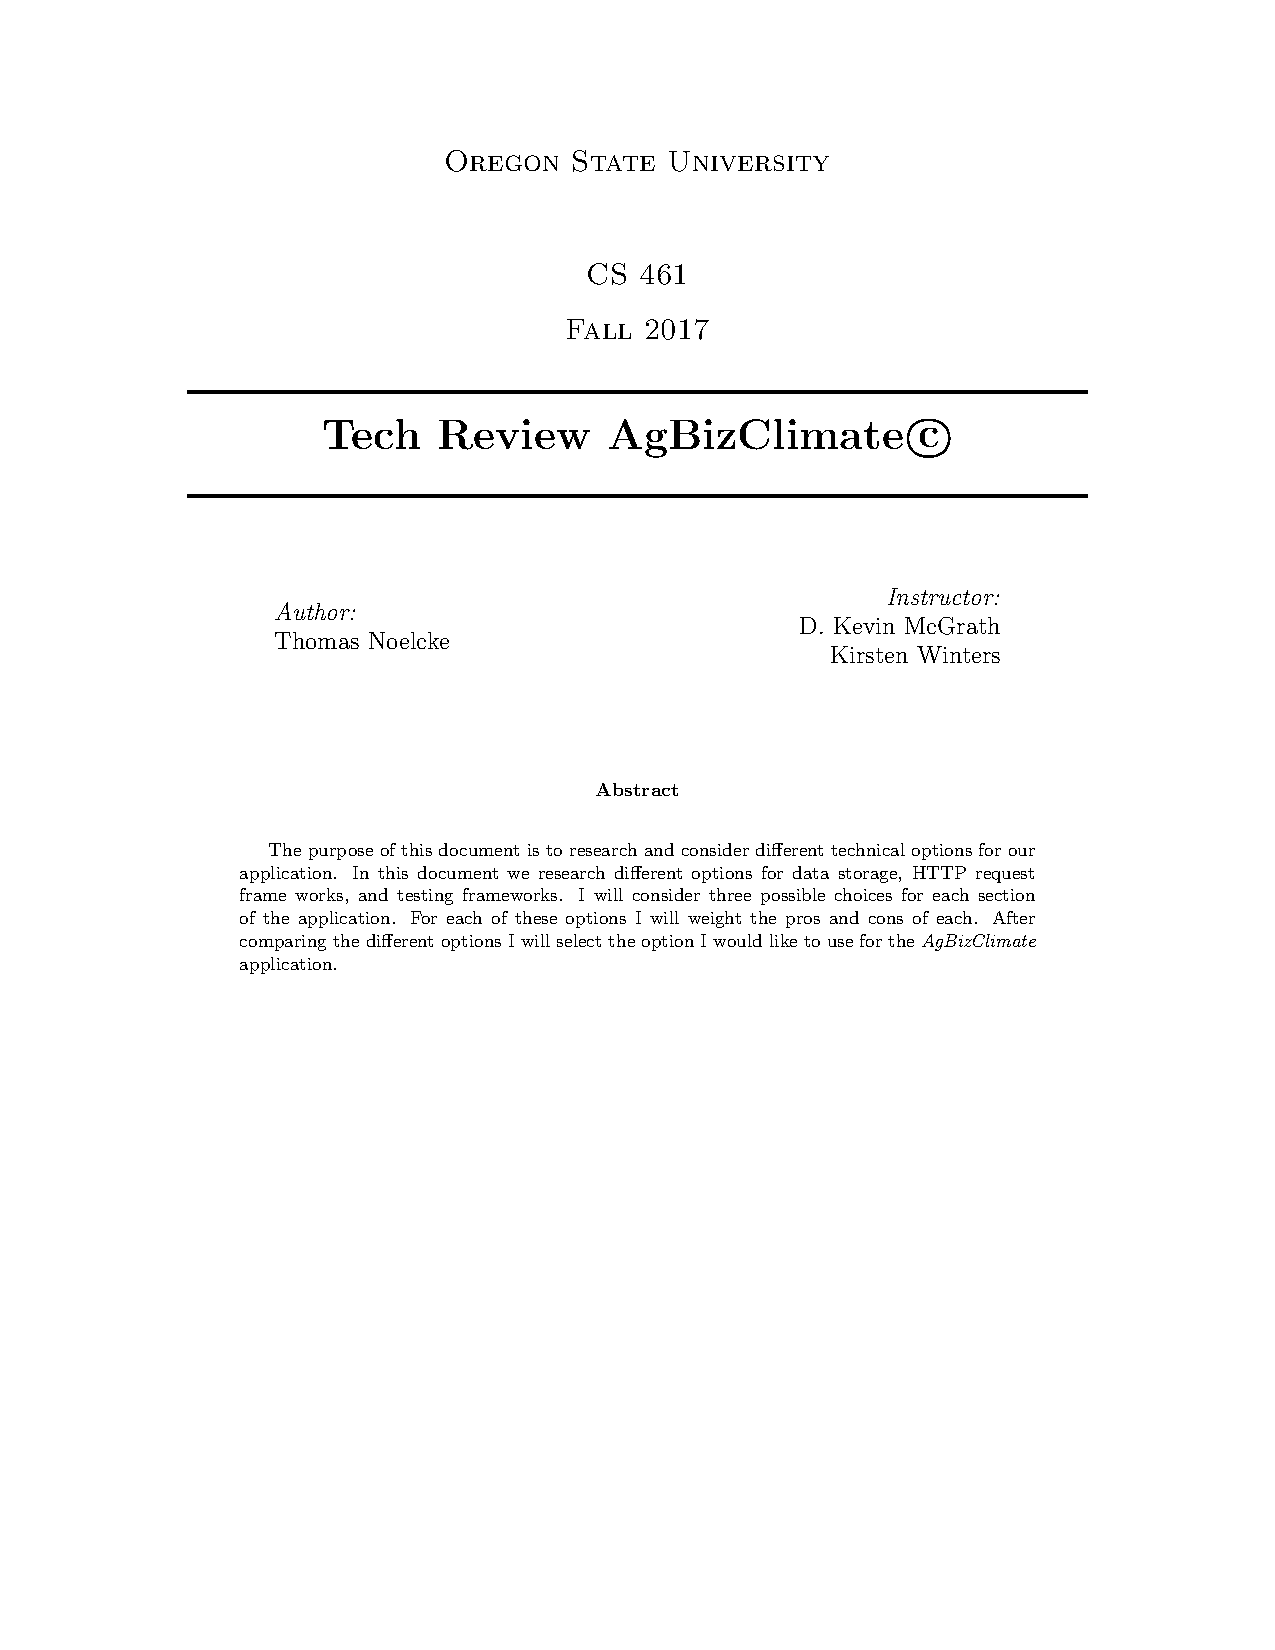
\includepdf[pages={1-8}]{Thomas/ThomasNoelckeTechReview.pdf}
		\section{Shengpei Yuan}
			
\includepdf[pages={1-5}]{Shengpei/main.pdf}
\end{document}